\documentclass{ximera}

\title{Creating Directional Derivatives from Partial Derivatives}
\author{Zack Reed}

\begin{document}
\begin{abstract}
We extend our understanding of derivatives from single-variable curves to multivariable surfaces by exploring how cutting through a surface's domain creates curves we can differentiate.
\end{abstract}
\maketitle

\section*{Simplifying the Directional Derivative: Losing Velocity Dependence}

As has been a theme of the course so far, we often get simpler, and at times more powerful, calculations and tools by losing dependence on time and velocity, instead focusing on undelrying geometric relationships.

This is also the case when it comes to differentiating multivariable functions! If we focus on geometric relationships, we not only simplify calculations by not needing to parametrize curves each time we want to take a derivative, but we also unlock very powerful tools that are fundamental to STEM.

We'll unpack this step-by-step. 

First, let's re-imagine directional derivatives in a slightly different way. The following video will summarize the main ideas, and you will then explore in the proceeding applet.

\begin{center}
\youtube{NGu7CSrHCvs}
\end{center}

\begin{expandable}{stuff}{GeoGebra Instructions}
 In this applet, you can move the blue black point on the left screen to change $(x,y)$. This changes where you're taking the derivative of $f$. You can also move the green dot at the end of the vector to change the direction in which you're taking the derivative. As you do so, note that a different curve is created on the 3D surface on the right.

For any given direction, if you select the ``Zoom to Differential'' button, the right screen will move close to the point on the surface and you can see the directional derivative vector. You can also check the ``Show Directoinal Derivative'' and ``Show Differential Build for dz'' boxes to see how the directional derivative is computed geometrically.
\end{expandable}

\begin{center}
\geogebra{gqa2xchz}{856}{440}
\end{center}

We're calling the tangent vector $df$ instead of the velocity. It's representing a small differential nudge along the surface in the direction specified. Also notice that we're calling the direction vector $ds$ instead of $\vec{u}$. This is because we're thinking of it as a small differential nudge in the domain.

If you just check the ``Show Directional Derivative'' box, you can see that the directional derivative vector is found by moving horizontally in the direction $ds$ and then moving up by the height change $dz$. 

The differential $dz$ is what we're really looking for when we take a directional derivative! We want to know at what rate the height changes as we move a small amount in the domain. One way to express this, as we've seen before, is that the differential change $dz$ is the product of the directional derivative and the distance moved in the domain:

$$dz = \frac{dz}{ds} \cdot ds$$

\begin{problem}

There is a very important relationship between $\frac{dz}{ds}$, $\frac{dz}{dx}$, and $\frac{dz}{dy}$ that we can use to simplify our calculations. See if you can figure it out by manipulating the applet and selecting the true statements from the following list:

\begin{selectAll}
\choice[correct]{If you move only in the $x$ direction, $\frac{dz}{ds}$ and $\frac{dz}{dx}$ are the same thing.}
\choice{The total height change $dz$ is independent of the height changes resulting from movement in the $x$ and $y$ directions.}
\choice[correct]{The total height change $dz$ depends on the height changes resulting from movement in the $x$ and $y$ directions.}
\choice[correct]{The height change after moving in the $x$ direction by some amount $dx$ is given by $\frac{dz}{dx} \cdot dx$.}
\choice{If you move only in the $y$ direction, $\frac{dz}{ds}$ is different from $\frac{dz}{dy}$.}
\choice{$\frac{dz}{ds}$ is the same as the velocity vector along the curve.}
\choice[correct]{The total height change $dz$ can be expressed as $dz = \frac{dz}{dx} \cdot dx + \frac{dz}{dy} \cdot dy$.}
\end{selectAll}

\begin{feedback}
Really play around with the applet and focus on the relationships between the variables. You'll want to hide and show different components as necessary to see the relationships, and you'll want to change the point and directions to confirm your understanding.
\end{feedback}
\end{problem}

\begin{remark}
Hopefully you've identified a key relationship: We can express any directoinal derivative entirely in terms of derivatives in the $x$ and $y$ directions!

We call these derivatives in the $x$ and $y$ directions \emph{partial derivatives}, and they are written as $\frac{\partial z}{\partial x}$ and $\frac{\partial z}{\partial y}$. We will spend much time learning to compute, understand, and learn partial derivatives in the coming sections.
\end{remark}



\section*{Why Partial Derivatives Are Nice}

Instead of parametrizing arbitrary curves through the domain, we can choose special curves that align with our coordinate system. This gives us partial derivatives naturally:

\begin{definition}

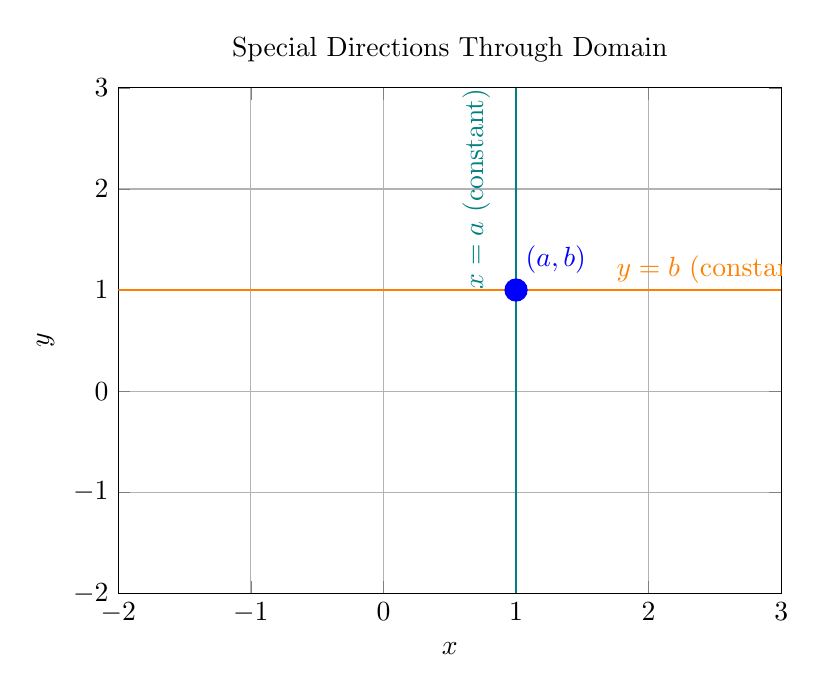
\begin{tikzpicture}
\begin{axis}[
    width=10cm,
    height=8cm,
    xlabel=$x$,
    ylabel=$y$,
    xmin=-2, xmax=3,
    ymin=-2, ymax=3,
    grid=major,
    major grid style={gray!60},
    title={Special Directions Through Domain}
]

% Point of interest
\addplot[only marks, mark=*, mark size=4pt, blue] coordinates {(1,1)};
\node[blue] at (axis cs:1.3,1.3) {$(a,b)$};

% Horizontal line (partial with respect to x)
\addplot[thick, orange, domain=-2:3] {1};
\node[orange] at (axis cs:2.5,1.2) {$y = b$ (constant)};

% Vertical line (partial with respect to y)
\addplot[thick, teal, domain=-2:3] ({1},x);
\node[teal, rotate=90] at (axis cs:0.7,2) {$x = a$ (constant)};

\end{axis}
\end{tikzpicture}

- **Orange line**: Moving in the $x$-direction only means that $y$ is constant. So we can take a derivative in $x$ just like we did in single-variable calculus.

We call this the \emph{partial derivative} of $f$ with respect to $x$, written $\frac{\partial f}{\partial x}$.


- **Teal line**: Moving in the $y$-direction only means that $x$ is constant. So we can take a derivative in $y$ just like we did in single-variable calculus.

We call this the \emph{partial derivative} of $f$ with respect to $y$, written $\frac{\partial f}{\partial y}$.

\end{definition}

\begin{problem}
Consider the function $f(x,y) = 3x^2y + y^3$ at the point $(2,1)$.

If we move in the pure $x$-direction, then we can treat $y$ as a constant (like $2$, or $\pi$ or $10$). The rate of change is:

$$\frac{\partial f}{\partial x} = \frac{\partial}{\partial x}[3x^2y + y^3] = \answer{6}xy + \answer{0} = \answer{6xy}$$

If we evaluate this derivative at the point $(2,1)$, we get:
$$\frac{\partial f}{\partial x}\bigg|_{(2,1)} = \answer{12}$$

If we move in the pure $y$-direction instead, then we can treat $x$ as a constant (like $2$, or $\pi$ or $10$). The rate of change is:

$$\frac{\partial f}{\partial y} = \frac{\partial}{\partial y}[3x^2y + y^3] = \answer{3}x^2 + \answer{3}y^2 = \answer{3x^2 + 3y^2}$$

If we evaluate this derivative at the point $(2,1)$, we get:
$$\frac{\partial f}{\partial y}\bigg|_{(2,1)} = \answer{15}$$

\begin{feedback}
If we treat $y$ as a constant, then we only need the power rule on $3x^2$, and $y^3$ is a constant so its derivative is $0$. Thus, $\frac{\partial f}{\partial x} = 6xy$, so at $(2,1)$: $6(2)(1) = 12$.

If we treat $x$ as a constant, then we only need the power rule on $y$ in both terms. Thus, $\frac{\partial f}{\partial y} = 3x^2 + 3y^2$, so at $(2,1)$: $3(2^2) + 3(1^2) = 12 + 3 = 15$.
\end{feedback}
\end{problem}

Let's do some more practice computing partial derivatives (derivatives in the $x$ and $y$ directions).

\begin{problem}
Compute the following partial derivatives and evaluate them at the given points.
\begin{enumerate}
  \item  If $f(x,y) = x^3y + y^2$ and $(x,y)$ is the point $(1,2)$ then 
  
  $$\frac{\partial f}{\partial x} = \answer{3x^2y}$$
  $$\frac{\partial f}{\partial x}\bigg|_{(1,2)} = \answer{6}$$

  \item If $f(x,y) = x^3y + y^2$ and $(x,y)$ is the point $(1,2)$ then
  
  $$\frac{\partial f}{\partial y} = \answer{x^3 + 2y}$$
  $$\frac{\partial f}{\partial y}\bigg|_{(1,2)} = \answer{5}$$

  \item If $f(x,y) = e^{xy} + x$ and $(x,y)$ is the point $(0,1)$ then
  
  $$\frac{\partial f}{\partial x} = \answer{ye^{xy} + 1}$$
  $$\frac{\partial f}{\partial x}\bigg|_{(0,1)} = \answer{2}$$
\end{enumerate}
\begin{feedback}
1. Treating $y$ as a constant, $\frac{\partial f}{\partial x} = 3x^2y$. At $(1,2)$: $3(1^2)(2) = 6$.
2. Treating $x$ as a constant, $\frac{\partial f}{\partial y} = x^3 + 2y$. At $(1,2)$: $(1^3) + 2(2) = 1 + 4 = 5$.
3. Treating $y$ as a constant, $\frac{\partial f}{\partial x} = ye^{xy} + 1$. At $(0,1)$: $(1)e^{0} + 1 = 1 + 1 = 2$.
\end{feedback}
\end{problem}

\section*{Any Direction You Want}

We'll return to the directional derivative later, after we've built up more tools for partial derivatives and related quantities, but for now we'll end by previewing the nice way to calculate directional derivatives using partial derivatives:

\begin{remark}
  If $\nabla f = \left\langle \frac{\partial f}{\partial x}, \frac{\partial f}{\partial y} \right\rangle$, and $\vec{u} = \langle u_1, u_2 \rangle$ is a unit direction vector, then the directional derivative of $f$ at a point in the direction of $\vec{u}$ is given by the dot product:

  $$D_{\vec{u}} f = \nabla f \cdot \vec{u} = \frac{\partial f}{\partial x} u_1 + \frac{\partial f}{\partial y} u_2$$

  The vector $\nabla f$ is called the \emph{gradient} of $f$, is very important.
\end{remark}

\end{document}